Here, we discuss the face code generation from numerical values of facial attributes. This is the most important and innovative module in our system and the first stage of \emph{face generation}. It's worth \textbf{noting} that we use both of the terms \emph{"feature"} and \emph{"attribute"} to refer to a facial attribute, like hair color or nose size.

\begin{figure}[H]
    \centering
    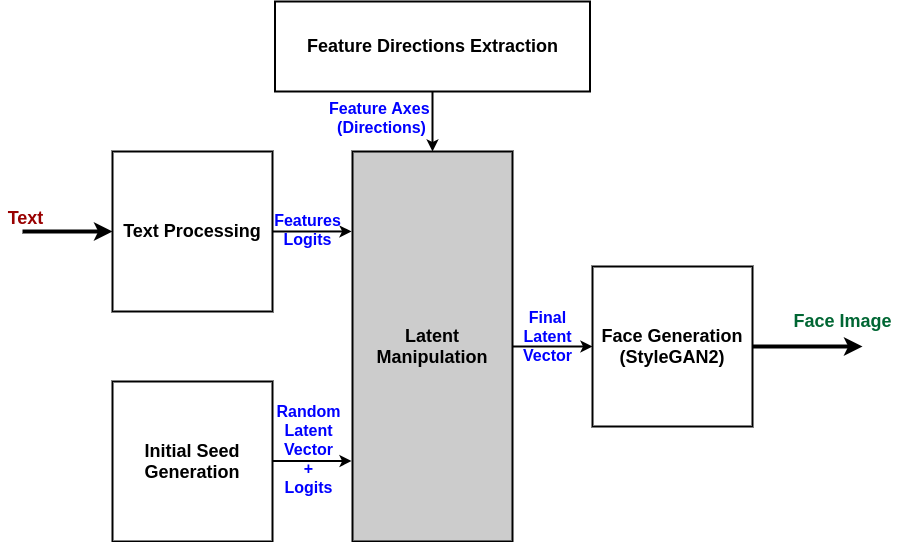
\includegraphics[width=0.8\textwidth]{images/face-gen-arch.png}
    \caption{Detailed block diagram of the three core modules workflow}
    \label{fig:face_gen}
\end{figure}

\subsubsection{Functional Description}

Figure \ref{fig:face_gen} shows a block diagram of the interaction between the $3$ core modules. We can see that the code generation module is the main driver of our face generation process. Generally, it converts the numerical attributes values (a.k.a. \emph{logits}) into a face embedding vector that matches the design of the latent space of the face generator (\emph{StyleGAN2}). Basically, it starts from an initial vector and uses the \emph{required feature values} and \emph{extracted feature directions} to transform this vector into the final latent vector, which is passed to the generative model.

\begin{itemize}
    \item \textbf{Input :}
    \begin{itemize}
        \item Numerical values of facial features (logits).
    \end{itemize}
    \item \textbf{Output :}
    \begin{itemize}
        \item Low dimensional face embedding vector (latent vector).
    \end{itemize}
\end{itemize}

\subsubsection{Modular Decomposition}

As figure \ref{fig:face_gen} tells, the code generation module can be torn down into $3$ sub-modules, which are \textbf{latent manipulation}, \textbf{initial seed generation} and \textbf{feature directions extraction}. Each sub-module is discussed in details to show how they integrate to each other to achieve the desired goal.

\paragraph{Feature Directions Generation}
Since, we use \texttt{StyleGAN2} \cite{karras2020analyzing} as our generative model, we have a full $512D$ latent space that is used to encode the whole face attributes. The changes in this latent space maps to the generated face image and similar features occupies the same area in the latent space. Consequently, we have to come up with a way to extract the axes (\emph{hyperplanes}) in this latent space to define each of our $32$ facial features. These feature directions are, then, used to manipulate the latent vector, in order to map to the required face image. 

\begin{figure}[H]
    \centering
    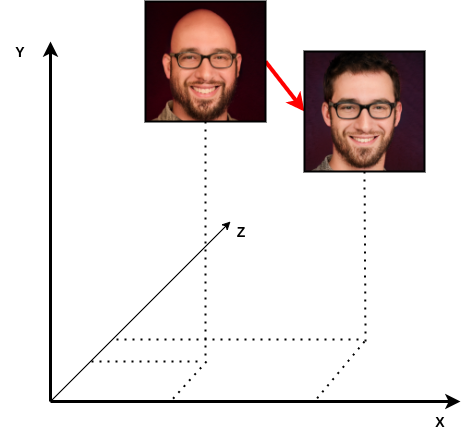
\includegraphics[width=0.5\textwidth]{images/feature-dir.png}
    \caption{Illustration of feature directions in latent space}
    \label{fig:feature_dir}
\end{figure}

Figure \ref{fig:feature_dir} further illustrates the idea of feature directions in the latent space. Here, we plot two face images in a $3D$ latent space. We can see that the difference between the two images in the existence and the absence of the hair, thus the red arrow represents the \emph{baldness} feature direction in that $3D$ latent space (moving along this particular vector causes hair density to change).

Our method of extracting the feature directions (\emph{hyperplanes}) consists of $3$ steps :
\begin{enumerate}
    \item \textbf{Code-Image Pairs Generation and Classification :} First, we use \texttt{StyleGAN2} to generate a large number of synthetic faces from random latent vectors. After so, we cluster the synthetic images (along with their latent vectors) according to each feature. The clustering can be based on discrete categories (like \emph{hair color} or \emph{race}) or continuous values (like \emph{hair length} or \emph{nose size}). We randomize the synthetic images in each clustering process to have better generalization and to cope with potential generation noise. For classification and regression, we use one of three possible methods, which are \textbf{manual labelling}, \textbf{classical image processing techniques} and \textbf{neural networks}. Thus, the output of this process is different groups of synthetic images sharing common facial features, along with their latent vectors.
    
    \item \textbf{Feature Directions Fitting :} Now, we have a set of latent vectors (\texttt{X}) and their corresponding feature values (\texttt{Y}). It's required to find a set of feature directions that satisfies the mapping between feature vectors and values. This problem can be formulated as :
    \begin{equation}
        Y = A_f \cdot X
    \end{equation}
    Where $A_f$ is the axis (direction) of feature $f$. \\
    We can obtain the solution to this equation in a closed form. However, due to the noise in both generation and classification, along with the non-linear nature of the problem, we opt to use \emph{ML} methods, specifically \textbf{Logistic Regression} and \textbf{SVM} to get an \emph{approximate solution}. Meanwhile, we cannot see any difference between the two methods, as they yield almost the same results. \\
    Finally, the generated feature directions are normalized to unit vectors :
    \begin{equation}
        A_{unit} = \frac{A}{||A||}
    \end{equation}
    
    \item \textbf{Directions Orthogonalization :} Facial features entanglement is one of the most difficult challenged of face generation. Some attributes in the human face tend to be extremely entangled by nature. For example, Asians rarely have curly hair, a woman cannot have beard and a man cannot put on makeup. Since \texttt{StyleGAN2} is trained and tuned on \textbf{FFHQ} dataset \cite{karras2019stylebased}, which contains real human faces, it is normal to notice some entanglement between some features. Consequently, the feature directions have to be further disentangled by using \emph{orthogonalization}. The orthogonalization process is done iteratively, starting from the most accurate feature directions. We orthogonalize other feature directions on the accurate ones, so that we have completely independent feature directions, where tuning one direction doesn't affect the others. The directions are orthogonalized as follows :
    \begin{equation}
        A_{proj} = (A \cdot B_{unit}) B_{unit}
    \end{equation}
    \begin{equation}
        A_{orthogonal} = A - A_{proj}
    \end{equation}
    
    Figure \ref{fig:ortho} visually illustrates the \emph{directions orthogonalization} process on $2D$ vectors.
    
    \begin{figure}[H]
        \centering
        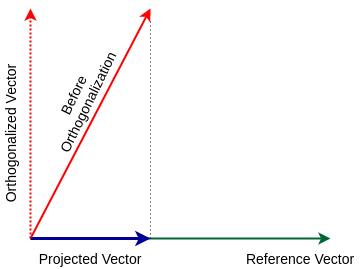
\includegraphics[width=0.5\textwidth]{images/orthogonalization.png}
        \caption{Illustration of orthogonalization relative to a reference vector}
        \label{fig:ortho}
    \end{figure}
    
    To ensure convergence to reasonable set of feature directions, we use a threshold margin to stop the orthogonalization process, which is from $85$ to $95$ degrees ($5$ degrees on each side of normal angle).
\end{enumerate}

\paragraph{Initial Seed Generation}
In order to avoid noise and discontinuities in the latent space, we generate an initial random latent vector. This is done by generating a random $512D$ vector and then passing it through the \emph{mapping network} of \texttt{StyleGAN2}, which is not invertible. This initial vector is, then, manipulated by sequential navigation along each feature direction (axis) with certain amounts. To get these amounts, we should know the component of the initial vector along each feature direction. We do that by simply performing a dot product between the initial vector and the unit vector of each feature direction. Thus, we have an initial latent vector and the numerical attributes values, it presents. 

\paragraph{Latent Manipulation}
This sub-module ingests all the inputs and produces the required latent vector (\emph{face embedding}) that describes all of the required facial attributes. The inputs to this latent manipulation sub-module are \emph{initial random vector} along with its logits, \emph{text logits} and \emph{feature directions}. The latent manipulation, simply, wants to realize the following transformation on the \emph{initial random vector} :
\begin{equation}
    E_{final} = E_{initial} + (l_{text} - l_{rand}) D
\end{equation}
Where $E_{final}$ is the final latent (\emph{embedding}) vector of dimensions $1X512$, $E_{initial}$ is the initial random vector of dimensions $1X512$, $l_{text}$ is the text logits vector of dimensions $1X32$ (remember that we consider $32$ facial features), $l_{rand}$ is the logits vector of the initial random vector of dimensions $1X32$ and $D$ is the feature directions matrix of dimensions $32X512$. The transformation includes calculating the difference between the required logits and the random logits and, then, use this difference to move the initial random vector along the feature directions to reach the final latent vector.

It might seem straight forward to perform this transformation. Unfortunately, it's not feasible to perform the transformation using direct matrix multiplication, mainly due to heavy \emph{entanglement} between direction vectors even after \emph{orthogonalization}. Also, the latent space of \texttt{StyleGAN2} can be very noisy in certain regions, so transformations have to be done carefully. 

Consequently, the processing in this sub-module is done iteratively as follows :
\begin{itemize}
    \item Both random and text logits are scaled from $0$ to $1$, which cannot have significant effect, when navigating using unit directions. Consequently, the inputs logits are scaled with the directions scale, which is obtained empirically to be from $-4$ to $4$, as shown in figure \ref{fig:dir_scale}.
    \item The next step is to get the \emph{difference} between \emph{text logits} and \emph{random logits}, which is of dimensions $1X32$. We call that \textbf{differentiated logits}. It's worth noting here that the input text usually contains a \emph{subset} of the facial features. Consequently, \emph{not all} the text logits are set to specific values. So, when doing the \emph{differentiation}, we set the differentiated logits of the \emph{unmentioned facial features} to $0$. So, it can be summarized as follows :
    \begin{equation}
        l_{diff}=
        \left\{ \begin{array}{ll}
            l_{text} - l_{rand} & l_{text} \neq None \\
            0 & \text{otherwise}
        \end{array} \right.
    \end{equation}
    \item Loop over each direction in feature directions :
    \begin{itemize}
        \item Multiply the \emph{differentiated logit} corresponding to the \emph{current feature} with its \emph{direction}.
        \item Add the product to the current latent vector (starting with the \emph{initial random vector}). The following equation summarizes these steps :
        \begin{equation}
            E_{next} = E_{prev} + l_{diff}[j] * D[j]
        \end{equation}
        \item Finally, to ensure that every transformation is independent of the subsequent transformations and that they are applied sequentially, we re-compute the \emph{produced latent vector logits} and re-differentiate it with the \emph{text logits}. This is done on every iteration of the latent manipulation process.
    \end{itemize}
\end{itemize}

\begin{figure}[H]
    \centering
    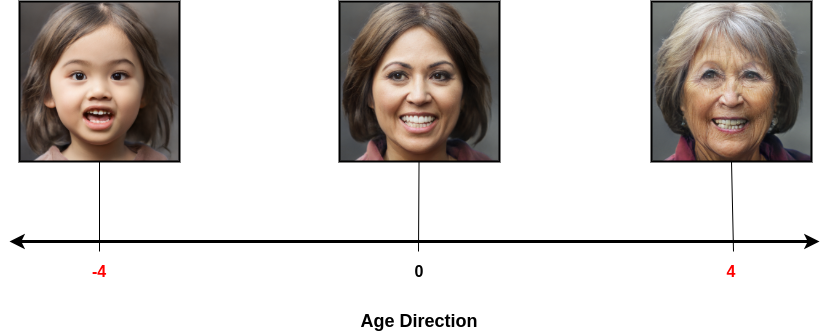
\includegraphics[width=0.8\textwidth]{images/dir-scale.png}
    \caption{Illustration of directions scale using age direction}
    \label{fig:dir_scale}
\end{figure}

By applying the previous process, the \emph{numerical value} of facial features extracted from text or manually entered by the user can be converted into a complete face embedding (\emph{latent vector}) matching the required facial attributes. This vector can be passed to \texttt{StyleGAN2} to translate it to a complete human face image.

\subsubsection{Design Constraints}

The design constraints of this module are enumerated as follows :
\begin{enumerate}
    \item \textbf{Facial attributes entanglement} is the main challenge of the face code generation module. Naturally, human face attributes are related to each other. For example, Asians barely have curly hair, no woman cannot have beard and most women have long hair and wear makeup. We mentioned before that \texttt{StyleGAN2} is trained and refined on \texttt{FFHQ} dataset, which contains real human faces. Consequently, it's normal to see heavy entanglement between features in the latent space. Due to this \emph{entanglement}, we have to perform extra computations to get decent results.
    \item \textbf{Random initialization} of the latent vector can cause some issues with the final output, as the vector can be initialized in a noisy area of the latent vector. We try to \emph{limit} the initialization of latent vector to a certain set of random vectors to avoid this effect. This method significantly reduces the \emph{random initialization effect}, however it's not fully cured.
    \item \textbf{Directions accuracy} can be a challenge as well. Some factors can negatively affect the feature directions accuracy. These factors include \textbf{synthetic image clustering} (whether \emph{classification} or \emph{regression}) and \textbf{directions fitting} process. We already discussed our solutions to this problem.
\end{enumerate}

\subsubsection{Synthetic Image Clustering}

As we mentioned before, it's required to cluster the generated synthetic images, in order to be able to fit the feature directions. The \emph{clustering} process can be performed through \emph{classification} or \emph{regression}. For example, features like hair and skin colors should be classified (grouped) into discrete categories, however features like hair length and mouth size should be assigned a continuous value. We do this task using one of three different methods :
\begin{enumerate}
    \item \textbf{Manual labelling} is the first idea to come to our minds. It's straight forward to manually classify a group of faces according to a certain feature. This method is used with some features, however it's very cumbersome and only works for classification.
    \item \textbf{Classical image processing techniques} are, also, used to classify images based on some features. Mainly, we use these techniques to detect \emph{colors} like eye color and hair color. We use \emph{morphological operators} and \emph{classical segmentation} to detect \emph{the eye} or \emph{the hair} and then retrieve its color.
    \item \textbf{Deep learning techniques} (\emph{neural networks)} are used to perform regression on the rest of the features. We basically use \emph{facial landmark detection} pretrained networks to detect the important facial landmarks, which is, then, used to calculate \emph{sizes} and \emph{distances}.
\end{enumerate}
